\documentclass[handout]{beamer}

%\usepackage[table]{xcolor}
\mode<presentation> {
  \usetheme{Boadilla}
%  \usetheme{Pittsburgh}
%\usefonttheme[2]{sans}
\renewcommand{\familydefault}{cmss}
%\usepackage{lmodern}
%\usepackage[T1]{fontenc}
%\usepackage{palatino}
%\usepackage{cmbright}

\useinnertheme{rectangles}
}
%\usepackage{normalem}{ulem}
%\usepackage{colortbl, textcomp}
\setbeamercolor{normal text}{fg = black}
\setbeamercolor{structure}{fg = blue}
\definecolor{trial}{cmyk}{1,0,0, 0}
\definecolor{trial2}{cmyk}{0.00,0,1, 0}
\definecolor{darkgreen}{rgb}{0,.4, 0.1}
\definecolor{mygray}{gray}{0.8}
\definecolor{myblack}{rgb}{0, 0, 0}
\usepackage{array}
\beamertemplatesolidbackgroundcolor{white}  \setbeamercolor{alerted
text}{fg=red}

\setbeamertemplate{caption}[numbered]\newcounter{mylastframe}

\usepackage{color}
\usepackage{tikz}
\usetikzlibrary{arrows}
\usepackage{colortbl}
%\usepackage[usenames, dvipsnames]{color}
%\setbeamertemplate{caption}[numbered]\newcounter{mylastframe}c
%\newcolumntype{Y}{\columncolor[cmyk]{0, 0, 1, 0}\raggedright}
%\newcolumntype{C}{\columncolor[cmyk]{1, 0, 0, 0}\raggedright}
%\newcolumntype{G}{\columncolor[rgb]{0, 1, 0}\raggedright}
%\newcolumntype{R}{\columncolor[rgb]{1, 0, 0}\raggedright}

%\begin{beamerboxesrounded}[upper=uppercol,lower=lowercol,shadow=true]{Block}
%$A = B$.
%\end{beamerboxesrounded}}
\renewcommand{\familydefault}{cmss}
%\usepackage[all]{xy}

\usepackage{tikz}
\usepackage{lipsum}

 \newenvironment{changemargin}[3]{%
 \begin{list}{}{%
 \setlength{\topsep}{0pt}%
 \setlength{\leftmargin}{#1}%
 \setlength{\rightmargin}{#2}%
 \setlength{\topmargin}{#3}%
 \setlength{\listparindent}{\parindent}%
 \setlength{\itemindent}{\parindent}%
 \setlength{\parsep}{\parskip}%
 }%
\item[]}{\end{list}}
\usetikzlibrary{arrows}
%\usepackage{palatino}
%\usepackage{eulervm}
\usecolortheme{lily}

\newtheorem{com}{Comment}
\newtheorem{lem} {Lemma}
\newtheorem{prop}{Proposition}
\newtheorem{thm}{Theorem}
\newtheorem{defn}{Definition}
\newtheorem{cor}{Corollary}
\newtheorem{obs}{Observation}
 \numberwithin{equation}{section}


\title[PLSC 43401] % (optional, nur bei langen Titeln nötig)
{Mathematical Foundations of Political Methodology Lecture 3}

\author{Robert Gulotty}
\institute[University of Chicago]{Department of Political Science \\  University of Chicago}
\vspace{0.3in}
\date{August 28th, 2017}

\setbeamertemplate{navigation symbols}{}

\begin{document}



\begin{frame}
\titlepage
\end{frame}



\begin{frame}{Sequences and Limits}
\begin{itemize}
\item We characterize the behavior of smooth functions with limits.
\item To understand a limit, we need to have a unit of account, which is a sequence.
\end{itemize}
\end{frame}


\begin{frame}

\begin{itemize}
\item \textcolor{myblack}{Sequence}

\item \textcolor{myblack}{Cauchy Sequence}
\item \textcolor{myblack}{Limits of Functions}
\item \textcolor{myblack}{Continuity}
\end{itemize}

\end{frame}



\begin{frame}

\begin{itemize}
\item \textcolor{myblack}{Sequence}
\item \textcolor{mygray}{Cauchy Sequence}
\item \textcolor{mygray}{Limits of Functions}
\item \textcolor{mygray}{Continuity}
\end{itemize}

\end{frame}


\begin{frame}
\frametitle{Sequence}

Sequence can be irregular, an example of such sequence is:

$$a_{1} = 1$$
$$a_{2} = 8$$
$$a_{3} = 6$$
$$a_{4} = ...$$

Sequence can be regular, an example of such sequence is:

$$x_{1} = 2$$
$$x_{2} = 4$$
$$x_{3} = 6$$
$$x_{4} = ...$$

\end{frame}

\begin{frame}
\frametitle{Sequence}

\begin{defn}
A \alert{sequence} of real numbers is a function, $u$, mapping $\mathbb{N}$ to $\mathbb{R}$
\end{defn} \pause

\begin{itemize}
\item We will be dealing with infinite sequences \pause
\item Written $u(1), u(2), u(3), ... $, or $(u_1, u_2, u_3, ...)$ \pause
\item The sequence is written $\{u_n\}$ \pause
\item For example: $$u_{n} = \frac{3n^2}{n^3+9}$$ gives the sequence $$\frac{3}{10}, \frac{12}{17}, \frac{48}{73}, ...$$
\end{itemize}
\begin{defn}
A \alert{sequence} of a set $X$ is a function, $u$, mapping $\mathbb{N}$ to $X$
\end{defn} \pause
\end{frame}


\begin{frame}
\begin{itemize}
\item Ideal classes of sequences:
\begin{itemize}
\item Arithmetic sequences
\item Geometric sequences
\end{itemize}
\item Defining characteristics of sequences
\begin{itemize}
\item Recurrent behavior: oscillation, convergence, divergence
\item Specific kinds of convergence.
\end{itemize}
\end{itemize}

\end{frame}




\begin{frame}
\frametitle{Arithmetic Sequences}

\begin{defn}
An arithmetic sequence is a sequence $\{u_n\}$ in which $$u_{n+1} - u_{n}$$ is constant for all $n$
\end{defn} \pause

\begin{itemize}
\item Equivalent to saying that for some numbers $a, d$, the sequence looks like $$a, a+d, a+2d, a+3d, ...$$ or $$u_n=a+(n-1)d$$ \pause
\item Is this sequence arithmetic? (If so, what are $a, d$?) $$u_{n} = 14 - 5n$$
\end{itemize}

\end{frame}



\begin{frame}
\frametitle{Geometric Sequences}

\begin{defn}
Geometric sequences: Each term is obtained by multiplying previous term by same number.
\end{defn} \pause

\begin{itemize}
\item Equivalent to saying that for some numbers $a, x$ the sequence looks like $$a, ax, ax^2, ax^3, ...$$ or $$u_n=ax^{n-1}$$ \pause
\item What are $a, x$ for this geometric sequence? $$u_n=5^{-n}$$ 
\end{itemize}

\end{frame}



\begin{frame}
\frametitle{Limits of Sequence: Motivation}

\begin{itemize}
\item Most sequences we will study will be neither arithmetic or geometric.\pause
\item How do we measure the behavior of sequences that change over time?   \pause
\item Many sequences behave similarly as $n$ gets large.
\item One way to characterize these sequences is to identify where they are converging to, a limit.
\item However, we need an objective criteria for determining whether two sequences are going to the same place.
\end{itemize}

\end{frame}




\begin{frame}
\frametitle{Sequence Applications}

\begin{itemize}
\item We saw that a sequence is some function $u(n)$ where $n$ is an integer.\pause
\item One important such function is:
$$u(1)=\frac{X_1}{1}$$\pause
$$u(2)=\frac{X_1+X_2}{2}$$\pause
$$u(3)=\frac{X_1+X_2+X_3}{3}$$\pause
$$u(n)=\frac{X_1+\ldots+X_n}{n}$$\pause

\item The sample average with increasing sample size will converge (in probability) to the true mean.
\end{itemize}

\end{frame}






\begin{frame}
\frametitle{Limits of sequences}

\begin{defn}
A sequence $\{ u_{n} \}$ tends to the limit $z$ if for any positive real number $\epsilon$ there exists a positive integer, $N$, such that:

$$|u_n-z|<\epsilon \hbox{ for all }n>N.$$\pause

Also written as  $$\lim u_n=z$$ $$\lim_{n\rightarrow \infty}u_n=z$$ $$u_n\rightarrow z \hbox{ as } n\rightarrow \infty$$
\end{defn}

\end{frame}



\begin{frame}
\frametitle{Limits of Sequences}

\begin{itemize}
\item Some Remarks
\begin{itemize}
\item If a sequence converges, it converges to one number, say $z$. \pause
\item We check by picking an $\epsilon>0$, which is an arbitrary real-valued number as the maximum deviation from the proposed limit $z$. \pause
\item Then we find the $N$, which will depend upon $\epsilon$, where the sequence is within the $\epsilon$ region of z.
\end{itemize}
\end{itemize}

\end{frame}



\begin{frame}
\frametitle{Limits of Sequences}

\begin{thm} $\left\{ \frac{1}{n} \right\}$ converges to 0 
\end{thm} 
\pause
\begin{proof}  Without loss of generality (WLOG) select an $\epsilon$.   We need 0 to be within $\epsilon$ of $N_{\epsilon}$:\pause
\begin{eqnarray}
|\frac{ 1} {N_{\epsilon}} - 0 | & < &  \epsilon  \nonumber \pause \\
\frac{1}{N_{\epsilon}} & < & \epsilon \nonumber\pause \\
\frac{1}{\epsilon} & < &  N_{\epsilon} \nonumber \pause
\end{eqnarray}
For each $\epsilon$, then, any $n> N_{\epsilon} > \frac{1}{\epsilon}$ will suffice.
\end{proof}\pause

\end{frame}


\begin{frame}

\begin{itemize}
\item \textcolor{mygray}{Sequence}
 
\item \textcolor{myblack}{Cauchy Sequence}
\item \textcolor{mygray}{Limits of Functions}
\item \textcolor{mygray}{Continuity}
\end{itemize}

\end{frame}

\begin{frame}
\frametitle{Cauchy, (pronounced KohShee) Sequence: Motivation}


\ \\In previous example, we could show that $\frac{1}{n}$ converges to 0 because we know its limit in advance. Can we show that a sequence has limit without knowing the limit \emph{ex ante}?\pause

\ \\A popular test for the existence of a limit is to determine if that sequence is Cauchy.



\end{frame}




\begin{frame}
\frametitle{Divergent Sequence}

\begin{defn}
A sequence that tends to a limit is called convergent; a sequence that doesn't is called divergent.
\end{defn} \pause

\begin{itemize}
\item A sequence that tends to infinity (or negative infinity) is divergent, but a sequence doesn't have to tend to infinity to be divergent. \pause (What's an example of a divergent sequence that doesn't tend to infinity?)
\end{itemize}

\end{frame}


\begin{frame}
\frametitle{Informal Definition of Cauchy Sequence}

A sequence  $\{x_{n} \}$ is Cauchy if it eventually stops bouncing around more than $\epsilon$:

\begin{itemize}
\item Find two points in the sequence $x_m$ and $x_n$.
\item Take their difference.  Is it getting smaller as m and n get big?
\end{itemize}


\end{frame}

\begin{frame}
\frametitle{Formal Definition of Cauchy Sequence}

\begin{defn}
A sequence $\{ u_{n} \}$ tends to the limit $z$ if $\forall \epsilon>0,\ \exists N\in \mathbb{N}:$\\ $|u_n-z|<\epsilon,\ \forall n>N.$\pause
\end{defn}

\begin{defn}
$\{x_n\} \hbox{ is Cauchy if } \forall\epsilon>0,\ \exists N\in \mathbb{N}:$\\$|x_{m} - x_{n}|<\epsilon \hbox{ when }m, n>N$
\end{defn}

\begin{thm}
In $\mathbb{R}$, $\{x_{n} \}$ is convergent if and only if it's Cauchy.
\end{thm}

\end{frame}


\begin{frame}
\frametitle{Apply Cauchy Criterion}

We can show the sequence defined by $x_1=1$, $x_2=2$,$\ldots$, $x_n=n$ is not convergent: \pause
\begin{itemize}
\item $|x_n-x_m|=|n-m|\geq 1$ for all $n, m$.\pause
\item Thus, for $\epsilon=1$ there is no $N$ such that $|x_n-x_m|<\epsilon$ whenever $n, m>N$.  \pause
\item  Therefore $\{x_n\}$ is not Cauchy, and does not tend to a limit.
\end{itemize}
\end{frame}



\begin{frame}
\frametitle{Working with Limits}

\begin{itemize}
\item Fact 1: For a real number $x$, $\lim_{n\rightarrow\infty}x^n=0$ if and only if $-1<x<1$. \pause
\item Fact 2: For a real number $b$, $\lim_{n\rightarrow\infty}n^b=0$ if and only if $b<0$.
%\item As $n\rightarrow \infty$, what's the limit of $$ u_{n} = {\frac{n+1}{2n}} $$
\end{itemize}

\end{frame}



%\begin{frame}
%\frametitle{Working with Limits}

%Claim: If $\lim u_n=z$ then $\lim |u_n |=|z|$ \pause

%\ \\Proof: If $\lim u_n=z$ then for any $\epsilon>0$,  $|u_n-z|<\epsilon$ for $n$ large. \pause  First, note that for real numbers $a, b$ we have $$||a|-|b||\leq |a-b|$$ (the ``reverse triangle inequality"). \pause This basically proves our result: For any $\epsilon >0$ we have $|u_n-z|<\epsilon$ for $n$ large, and consequently $||u_n|-|z||<|u_n-z|<\epsilon$.  Thus, $\lim |u_n |=|z|$. $\Box$ \pause

%\ \\Does the converse hold? (If $\lim |u_n |=|z|$  then $\lim u_n=z$)

%\end{frame}



\begin{frame}
\frametitle{Working with Limits: Evaluate Dominating Term}

What is the limit of 
$$ u_{n} = \frac{(-1)^n (n+1)^2}{n^4} $$

\ \\Hint: We can start by expanding the numerator. \pause
$$ u_{n} = \frac{(-1)^n (n^2+2n+1)}{n^4} $$\pause
$$ u_{n} = \frac{(-1)^n (n^2)}{n^4}+\frac{(-1)^n (2n)}{n^4}+\frac{(-1)^n}{n^4} $$\pause
\ \\What would happen if we replaced $(n+1)^2$ with $(n+1)^4$?  \\Don't do whole calculation! \pause
\end{frame}






\begin{frame}
\frametitle{Working with Limits: Evaluate Dominating Term}
Another practice, though easier one, as $n\rightarrow \infty$, what's the limit of 
$$ u_{n} = {\frac{n+1}{2n}} $$\pause

$$ u_{n} = \frac{n}{2n}+\frac{1}{2n} $$\pause
$$ u_{n} = \frac{1}{2}+0 $$


\end{frame}



\begin{frame}
\frametitle{Series}
\begin{defn}
A \alert{series} is sequence constructed from a sum of sequences.
\end{defn} \pause
\begin{itemize}
\item The series defined by a sequence $\{u_n\}$ is the sequence $\{s_n\}$ with $$s_1=u_1, s_2=u_1+u_2, s_3=u_1+u_2+u_3, ...$$ and more generally $$s_n=\sum_{r=1}^{n}u_r$$ \pause

\item Thus, series is a special type of sequence, it sums the terms in the sequence.
\end{itemize}

\end{frame}


\begin{frame}
\frametitle{$\sum$ notation for series}

$$s_n=\sum_{r=j}^{n}u_r$$
Here $j$ is the start of the series, $n$ is the end.  We work through each number from $j$ to $n$, plugging into $r$.\pause
\vspace{5mm} \\ 
Suppose $j=0$, $n=10$ and $u_r = 2* r$ 

$$s_n=\sum_{r=0}^{10}u_r=0+2+4+6+8+10+12+14+16+18+20$$
$$=\sum_{r=0}^{3}u_r+\sum_{r=4}^{7}u_r+\sum_{r=8}^{10}u_r$$

\end{frame}

\begin{frame}
\frametitle{Formula for Summing Algebraic Sequence}

\ \\We are interested in the sum of first $n$ terms in arithmetic sequence. Here is the derivation: \pause

\ \\First, the natural numbers $$s_n=1+ 2+ ...+(n-1)+  n$$
 $$s_n=n + (n-1) + ...+ 2+ 1$$ \pause
 
 Adding these together we get 
 
 $$2s_n=(1+n)+(1+n)+...+(1+n)= n(1+n)$$ \pause
 
 The first $n$ terms of the natural numbers sum to 
 $$s_n={\frac{1}{2}}n(1+n)$$

\end{frame}



\begin{frame}
\frametitle{Formula for Summing Algebraic Sequence}

Recall that a general arithmetic sequence is $u_n=a+(n-1)d$ \pause

\ \\We can use the same trick to find the sum of the first $n$ terms of the sequence:

$$u_n=a+(a+d)+(a+2d)+...+(a+(n-2)d)+(a+(n-1)d)$$\pause
$$u_n=(a+(n-1)d)+(a+(n-2)d)+...+(a+2d)+(a+d)+a$$\pause
$$2u_n=n\left(2a+(n-1)d\right)$$\pause
$$2u_n=2an+n(n-1)d$$\pause
$$u_n=an+n\left({\frac{(n-1)d}{2}}\right)$$

\end{frame}



\begin{frame}
\frametitle{Summing Geometric Sequences}
These same tricks can be extended to the geometric sequence:
$$s_n=a+ax+ax^2+...+ax^{n-1}$$ \pause
Our strategy is to construct a forward and backward shifted sequence and then take differences to eliminate the middle.\pause
\ \\Multiplying by $x$ we get our original sequence shifted forward.
$$xs_n=ax+ax^2+...+ax^n$$ \pause
We then define a sequence for all but the first term.
$$t=ax+ax^2+...+ax^{n-1}$$ \pause 
Then $s_n=a+t$ and $xs_n=t+ax^n$, we can eliminate $t$.  
\begin{eqnarray}
s_n-xs_n&=&a-ax^n \nonumber\\ \pause
s_n(1-x)&=&a(1-x^n) \nonumber\\ \pause
s_n &=& a\left({\frac{1-x^n}{1-x}}\right)  \nonumber
\end{eqnarray}

\end{frame}



\begin{frame}
\frametitle{An Example for Summing Geometric Sequence}

\ \\Now suppose you save \$1000 in Citibank this year. Every future year, you save \$1000. The annual (compound) interest rate is 5 percent. \pause

\ \\Then, a natural question will be: at year $n$, how much money do you make? \pause

\ \\For the money you saved at year $0$, you will get: $1000 * (1 + 0.05)^{n}$; \pause

\ \\For the money you saved at year $1$, you will get: $1000 * (1 + 0.05)^{n-1}$; \pause

\ \\For the money you saved at year $t$, you will get: $1000 * (1 + 0.05)^{n-t}$; \pause

\ \\Sum them together and you will have your total earnings: 
$$1000 * (1 + 0.05)^{n} + 1000 * (1 + 0.05)^{n-1} + ... + 1000 * (1 + 0.05)^{1}=13,206.79$$

\end{frame}

\begin{frame}
\frametitle{Utility Application of Geometric Series}
\begin{itemize}
\item Geometric series are often used to study the value of the future:
\item $U(a)=a+a\delta+a\delta^2+...+a\delta^{n-1}$ \pause
\item $\delta$ is called the discount factor, and  $0<\delta<1$ \pause
\item We can use the properties of series to describe the long run (infinite) value of a choice.
\end{itemize}

\end{frame}

\begin{frame}
\frametitle{Convergence of Geometric Series}

\ \\For a geometric series, $$s_n=a\left(\frac{1-x^n}{1-x}\right)$$ \pause

\ \\We know that $x^n\rightarrow 0$ as $n\rightarrow\infty$ if and only if $|x|<1$ \pause

\ \\If $|x|<1$ then $\lim_{n\rightarrow\infty}s_n = a\left({\frac{1-0}{1-x}}\right) = {\frac{a}{1-x}}$\pause

\ \\ Applying this result to the long run value of a: $U(a)= \frac{a}{1-\delta}$.
$$\sum_{t=0}^\infty \delta^t u(x) = {\frac{u(x)}{1 - \delta}}$$

\end{frame}



\begin{frame}
\frametitle{Divergence of Geometric Series}

\ \\Recall that $s_{n} = \sum_{n = 1}^{\infty} k_{n}$. \pause

\ \\Fact (\textit{term test} for any series): If $\lim_{n\rightarrow \infty} k_n\not=0$ then $\sum_{n=1}^\infty k_n$ diverges \pause

\ \\For a geometric series, $k_n=ax^{n-1}$ \pause

\ \\We know that $x^n\rightarrow 0$ as $n\rightarrow\infty$ \underline{if and only if} $|x|<1$ \pause

\ \\Therefore, a geometric series diverges whenever $|x|\geq 1$

\end{frame}




\begin{frame}

\begin{itemize}
\item \textcolor{mygray}{Sequence}
 
\item \textcolor{mygray}{Cauchy Sequence}
\item \textcolor{myblack}{Limits of Functions}
\item \textcolor{mygray}{Continuity}
\end{itemize}

\end{frame}



\begin{frame}
\frametitle{Limits of Functions: Motivation}


\begin{figure}[!ht]
\centering
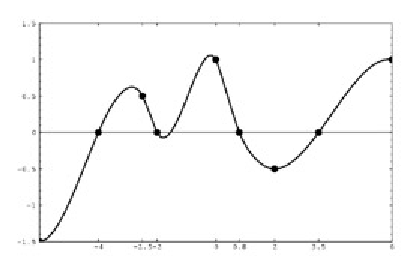
\includegraphics{plsc43401_lec2_pic1}
\end{figure}

\ \\We care about the limits of function because we care about how functions behave at a point. \pause
\ \\It turns out that function can often only be described in the limit (recall probability example).


\end{frame}



\begin{frame}
\frametitle{Limits of Functions}

\begin{defn}
Suppose $f: \mathbb{R} \rightarrow \mathbb{R}$.  We say that $f$ has a limit $L$ at $x_{0}$ if, for each $\epsilon>0$, there is a $\delta>0$ such that $|x - x_{0}|< \delta$ implies that $|f(x) - L| < \epsilon$.  
\end{defn} \pause

\begin{itemize}
\item Limits are about the behavior of functions at points.  Here $x_{0}$. \pause
\item As with sequences, we let $\epsilon$ define an error rate \pause
\item $\delta$ defines an area around $x_{0}$ where $f(x)$ is going to be within our error rate
\end{itemize}

\end{frame}



\begin{frame}
\frametitle{Limits of Functions: Example}

\begin{thm}
The function $f(x) = \frac{x^2 - 1}{x - 1} $ has a limit of $2$ at $x_{0} = 1$.  
\end{thm} \pause

\textbf{Proof step 1, simplify}\\
For all $x \neq 1$, 
\begin{eqnarray}
f(x)&=&\frac{x^2 - 1}{x - 1} \nonumber \\	
 & = & \frac{(x + 1)(x - 1) }{x - 1}  \nonumber \\					
								& = & x + 1 \nonumber 
\end{eqnarray} 

\end{frame}

\begin{frame}{Limits of Functions: Example Continued}
Show $f(x) = \frac{x^2 - 1}{x - 1} =x+1$ has a limit of $2$ at $x_{0} = 1$.\\
 
\textbf{Proof step 2:}\\\pause
Choose any $\epsilon >0$ and set $x_{0}=1$.  We're looking for $\delta_{\epsilon}$ (a function of $\epsilon$) such that 
\begin{eqnarray}
|x - 1|< \delta_{\epsilon} & \text{ implies } & |(x + 1) - 2| < \epsilon \nonumber 
\end{eqnarray} \pause
We guess a good $\delta_{\epsilon}$ and use a direct proof:\\
Assume $\delta_{\epsilon} = \epsilon$,\pause  
$$|x - 1|< \delta_{\epsilon}$$
$$|x - 1|< \epsilon$$\pause
$$|x +(1-1) - 1|< \epsilon$$\pause
$$|(x +1)- 2|< \epsilon$$		

\end{frame}

\begin{frame}
\frametitle{Remarks on Limits of Functions}

\ \\$\lim_{x\rightarrow x_o}f(x)$ might or might not equal $f(x_o)$ \pause

\begin{itemize}
\item It could be \textit{different than} $f(x_o)$ \pause

 \[
    f(x)=\left\{
                \begin{array}{lll}
                  +1&\hbox{if } x\not=4\\
                  -1&\hbox{if } x=4
                \end{array}
              \right.
  \] \pause

%$\lim\limits_{x\rightarrow 4}f(x)=1$ while $f(4)=-1$

\item It could be \textit{undefined} \pause

 \[
    f(x)=\left\{
                \begin{array}{lll}
                  +1&\hbox{if } x<0\\
                  -1&\hbox{if } x\geq 0
                \end{array}
              \right.
  \]

\end{itemize}

\end{frame}



\begin{frame}
\frametitle{Example of Cauchy sequence}
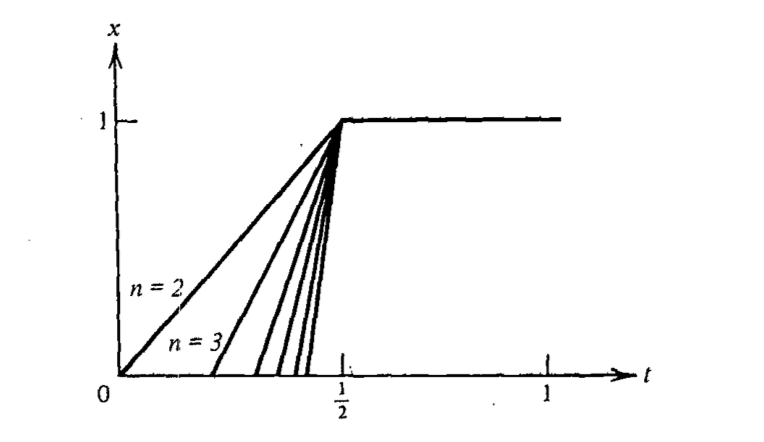
\includegraphics[width=4 in]{CauchyFun.png}

\begin{itemize}
\item Suppose $x_n(t)=\begin{cases}0 & \quad \text{for } \quad 0\leq t\leq\frac{1}{2}-\frac{1}{n}\\ nt-\frac{n}{2}+1& \quad \text{for } \quad \frac{1}{2}-\frac{1}{n}\leq t \leq\frac{1}{2}\\ 1& \quad \text{for } \quad t\geq \frac{1}{2} \end{cases}$
\end{itemize}

\end{frame}


\begin{frame}
\frametitle{Algebra of Limits}

\begin{thm}
Suppose $f:\mathbb{R} \rightarrow \mathbb{R}$ and $g: \mathbb{R} \rightarrow\mathbb{R}$ with limits $A$ and $B$ at $x_{0}$.  Then, 
\begin{eqnarray}
\text{i.) } \lim_{x \rightarrow x_{0} } (f(x) + g(x) ) & = & \lim_{x \rightarrow x_{0}} f(x) + \lim_{x \rightarrow x_{0}} g(x)  = A + B\nonumber \\\pause
\text{ii.) }\lim_{x \rightarrow x_{0} } f(x) g(x) & = & \lim_{x \rightarrow x_{0}} f(x) \lim_{x\rightarrow x_{0}} g(x)  = A B\nonumber 
\end{eqnarray}
Suppose $g(x) \neq 0$ for all $x \in \mathbb{R}$ and $B \neq 0$ then $\frac{f(x)}{g(x)}$ has a limit at $x_{0}$ and 
\begin{eqnarray}
\lim_{x \rightarrow x_{0}} \frac{f(x)}{g(x)} & = &  \frac{\lim_{x\rightarrow x_{0} } f(x) }{\lim_{x \rightarrow x_{0} } g(x) } = \frac{A}{B}\nonumber 
\end{eqnarray}
\end{thm}

\end{frame}



\begin{frame}
\frametitle{Power Series}

\begin{itemize}
\item The following is the most important function in mathematics:\pause
$$e^x=\sum_{n=0}^{\infty} \frac{x^n}{n!}=\lim_{n\rightarrow \infty} \left(\frac{1}{0!}+\frac{x}{1!}+\frac{x^2}{2!}+... +\frac{x^n}{n!}\right)$$\pause
\item It has special properties when we get to derivatives.
\end{itemize}

\end{frame}



\begin{frame}

\begin{itemize}
\item \textcolor{mygray}{Sequence}
\item \textcolor{mygray}{Cauchy Sequence}
\item \textcolor{mygray}{Limits of Functions}
\item \textcolor{myblack}{Continuity}
\end{itemize}

\end{frame}



\begin{frame}
\frametitle{Continuity} 

\begin{defn}
Suppose $f:\mathbb{R} \rightarrow \mathbb{R}$ and consider $x_{0} \in \mathbb{R}$.  We will say $f$ is continuous at $x_{0}$ if for each $\epsilon>0$ there is a $\delta>0$ such that if, 
\begin{eqnarray}
|x - x_{0} | & < & \delta \text{ for all  } x \in \mathbb{R}\text{ then } \nonumber \\
|f(x) - f(x_{0})| & < & \epsilon \nonumber 
\end{eqnarray}
\end{defn} \pause

\begin{itemize}
\item Previously $f(x_{0})$ was replaced with $L$. \pause
\item Now: $f(x)$ has to converge on itself at $x_{0}$. \pause 
\item Continuity is more restrictive than limit.
\end{itemize}

\end{frame}


\begin{frame}
\frametitle{The intermediate value theorem}
Consider an interval $[ a,\ b ]$ in the real numbers.
\ \\If the function $f(x)$ is continuous for all $a\leq x\leq b$ then $f$ takes every value between $f(a)$ and $f(b)$.

\begin{center}
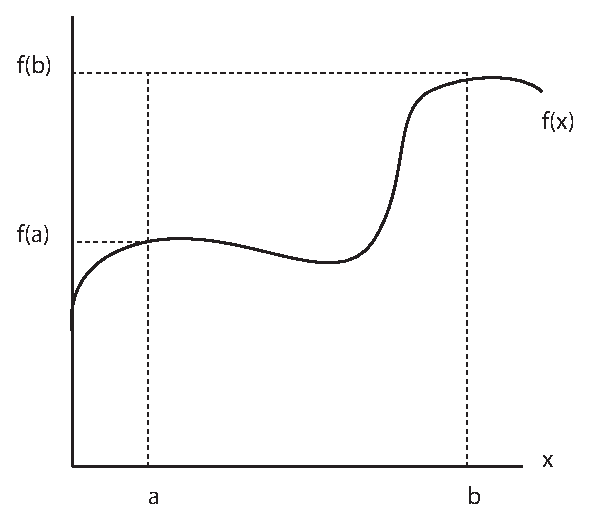
\includegraphics[width=2.5 in]{intVal.eps}
\end{center}

\end{frame}



\begin{frame}
\frametitle{Proof outline of intermediate value theorem}
\begin{itemize}
\item If we have any $u$ between two values of the function, $f(a)$ and $f(b)$, we can find a $f(c)=u$
\item Call S the set of numbers $x\in [a,\ b]$ such that $f(x)\leq u$.  We want to show that the function takes on the value $f(c)=u$ at some $c \in S$.  We will show that this occurs at the supremum (the lowest number greater than or equal to every element of S). 
\item Pick a small area around $f(x)$, use properties of continuity of $f$ and the real numbers, find that the only value that can satisfy these conditions is $f(c)=u$
\end{itemize}

\end{frame}











\end{document}
